\section{Computer Experiments} \label{ch:computer_experiments}
This section describes the setup and configuration of the computational experiments conducted in this study, and the accompanied results. Two types of statistical models, \acrshort{convlstm} and \acrshort{ar}-model are trained and evaluated on an unseen portion of the dataset. 

\subsection{Framework, Structure and Implementation} \label{sec:structure_and_implementations} \label{sec:framework}
%\section{Structure and Implementations} 
The numerical methods used in this study are described in Chapter \ref{ch:num_methods}. The code is available on GitHub in the project repository named ``MS'' on \href{https://github.com/hannasv/MS}{https://github.com/hannasv/MS}. Instructions for downloading 
reanalysis (ERA5) data using python is provided. 
The dataset is not published because of a licences on the \acrshort{msg} data. 
%Due to licence requirements on the \acrshort{msg} data, no part of \acrshort{ecc} is made available for downloading. %The reader need to aquire their own \acrshort{msg} data throught the eumetcast portal and can regridd the product using the code made availble.

%\textbf{Due to liscence on the MSG data in finer than X resolution, the full dataset is not made aailable. The code for regridding and thedescriptions for downloading the data is made available.}



%The repository contains everything need to reproduce the results in this study.
%The experiments are conducted in notebooks and the developed modules are stored in the package ``sciclouds''. Descriptions on how to acquire the data (scripts if possible) and project environment is provided to simplify the process.

The code is developed in Python 3.7, a popular language for scientific software development. The source code is stored in the package \textit{sciclouds}, made available on Github through the project repository. Developed modules draw inspiration from the structure of \textit{scikit-learn} (\cite{sklearn_api}).
%and the \textit{keras-tuner} (\cite{chollet2015kerastuner}). 
%The \acrshort{convlstm} is implemented %in \textit{keras} (\cite{chollet2015keras})
%using \textit{tensorflow v 2.0} . %The \textit{keras-tuner} is used to automize the hyperparameter search (\cite{chollet2015kerastuner}). 
The \acrshort{convlstm} is implemented using Tensorflow's keras API (\cite{tensorflow2015}) which simplifies many aspects of building and executing machine learning models. To utilize the analytical solution the \acrshort{ar}-models are trained and evaluated using self implemented modules.
%The \acrshort{ar}-models are trained and evaluated using self implemented modules. The idea was to utilize the analytical solution of the least squares problem. 
%Many regression modules provide a numerical solution, not the analytical. 
The python package ``sclouds'' provides a self implemented version of \acrshort{ar}-models, using the analytical solution to the least squares problem derived in Section \ref{sec:ARmodels}.

Visualizations are generated using \textit{Matplotlib} (\cite{matplotlib}),  \textit{Seaborn} (\cite{seaborn}) and maps using the package \textit{Cartopy} (\cite{Cartopy}). Other illustrations are developed using TIkZ, a language used for producing technical illustrations within the environment of LaTeX.

The package versions are documented in the \textit{requirements.txt} and the project environment called ``sciclouds'' is ready for installation. This is a conda environment, the yaml-file lists the Python packages and requirements necessary for running this code. Below you find the code example for cloning the project and installing the environment.

% Included in the readme file on github. 
\begin{verbatim}
git clone https://github.com/hannasv/MS.git
cd MS
conda env create -f environment.yml
conda activate sciclouds
python setup.py install # installing package from source
\end{verbatim}

Supplementary material for remapping satellite data and filtering masks is available in the supplementary repository \href{https://github.com/hannasv/MS-suppl}{https://github.com/hannasv/MS-suppl}. %To make use of all the functionality available trought ``MS'', the supplementary repository needs to be cloned in the same directory.
The filters are generated from within the environment of PyAEROCOM (\cite{pyaerocom}). 


%Complex computations will cause memory growth, dependant on how many intermediate computations it needs to store. This is the case for \acrshort{convlstm}. To speed up the development process the software is developed on a subset of \acrshort{ecc}. Small adjustments needs to be made, running experiments on the entire data. For instance threads deadlock when extracting large amounts of data. This is a precautionary measure to avoid overloading the system. \textbf{Possible to develop code to do Hyperparameter tuning based on }
%For a more detailed description please see the project repository described in Section \ref{sec:structure_and_implementations}.

\subsection{Hardware} \label{sec:hardware}
%How to deal with big datasets that will easily eat up you memory? ``Big data'' involve processing large amounts of data that does not fit into memory. Processing substantial amounts of data require expert knowledge about distributed systems and analysing for system bottlenecks.  %Although theoretically fascinating it remains to see if \acrshort{convlstm} provide a clear practical advantage over the autoregressive models.
%Conducting experiments on big datasets require external computational resources.  
The experiments described below, are conducted on a 
%This study had access to a 
DGX-2 system consisting of 16 NVIDIA Tesla V100 GPUs, each of 32Gb local memory and 1.5Tb shared memory. %The resources was available through the \acrfull{ex3} project hosted at Simula. 
%This study was awarded access to 1 GPU and 1024G part of the memory. 
The data is stored on a \acrfull{rdma} accessed over Infiniband. %\textit{The best choice of collective implementation depends upon the number and kind of \acrshort{gpu}s, and the network interconnect in the cluster.} 
The DGX-2 system is designed for a high level concurrency and scheduling workers competing for system resources.
%The hardware sets the limitations for efficiency of pipelines and training procedure. 
%\textit{NVIDIA V100 GPU -- The eX3 infrastructure includes a DGX-2 system consisting of 16 NVIDIA Tesla V100 GPUs, allowing simultaneous communication between all eight GPU pairs at 300 GBps through the 12 integrated NVSwitches. This gives a theoretical system-wide system bi-directional  bandwidth of 2.4 TBps. All GPUs have 32 GB of local memory (total of 512 GB) and share a 1.5 TB main memory. The total system has 81,920 CUDA cores, and 10,240 Tensor cores delivering 2 Petaflops of tensor performance. The peak performance in double precision is 125 Teraflops.}
%Working on such a monstrosity pose additional challenges related to porting existing code and virtual environments, developing and debugging code. To eventually end up with an%a achieved 
%acceptable level of efficiency and reliability. \textbf{må de siteres? (\cite{ex3docs} and \cite{ex3homepage}).} 
\begin{table}[ht]
    \centering
    \begin{tabular}{c|c}
        Device &  Type  \\ \hline
        GPU & Tesla V100-SXM3-32GB \\
        CPU & DualProcessor AMD Epyc7601 (SMT2) w/2TB ram and 4TB NVMe 
    \end{tabular}
    \caption{Hardware specifications for the environment used on \acrshort{ex3}. The operating system is Ubuntu 18.04.4.}
    \label{tab:hardware_ex3}
\end{table}
%\textbf{TS: Mye av teksten frem til dette punktet egner seg egentlig bedre i et Appendix}
%TS: Mye av teksten frem til dette punktet egner seg egentlig bedre i et Appendix
\subsection{Model Setup and Evaluation}
The following sections contain the configurations of the models compiled for this study, along with descriptions of hyperparameters. A model is pieced together based on a set of hyperparameteres. This includes parameteres set prior to training, as mentioned in Section \ref{sec:artificial neural networks}.

%A model is compiled based on a choice of hyperparameters. It is a set of decisions made prior to training, as mentioned in Section \ref{sec:artificial neural networks}.
In the search for the best model configuration, different combinations of hyperparameters are evaluated based on the metric, \acrfull{mae}. In this study the tuning was performed manually since the choice of architecture easily overload the system memory resources. The \acrshort{ar}-models follow a strategy, building the simplest models first and gradually increasing the complexity. The set of architectures provided by \citeauthor{SunAirLSTM} (\citeyear{SunAirLSTM}), described in Section \ref{sec:related_work}, serve as a starting point for \acrshort{convlstm} built in this study.  %This could have been done using spaced sampling, attempting lags of 1, 2, 5, 10. The result becomes the same, however for large model there might be some time to save.

%it follows the principal of starting with the simplest model possible and increasing the complexity from there. 
%Stopping at architectures where increased complexity don't increase the performance? Know stategies are using spaced sampling, attempting lags of 1, 2, 5, 10. The second is naturally to further investigate regons of lags showing the most promise. 
%on a similar problem, air quality forecasting problem was executed. \citepaper{chollet2015kerastuner} provide suitable software for the automatic hyperparameter tuning. 
%\textbf{Man kjører eksperimenter på mange modeller ved å bruke traning og validations dataset. The choice of model is based on this data basis and then it performance is tested on the test dataset.} 
\subsection{Training, validation and test split}
Gradient methods are at the heart of every machine 
learning algorithms. It is based on the principle that the model is continuously evaluated against the validation dataset and weights are adjusted to reduce the loss. This raises the need for two potions for training. The \acrshort{ar}-models are computed based on an analytical solution and have no need for a validation set. 

Based on the assumption that the most resent partition is representative for the near future, both models are tested on 2014 to 2018. The \acrshort{ar}-model is trained on the period 2004 to 2013, while the \acrshort{convlstm} is trained on  2004 to 2011 and validated on 2012 to 2013.

%&Therefore the evaluation on this portion is as close one get to evaluate on future climates.
%Which is a important aspect when we 
%Da får vi et best mulig riktig inntrykk av hvordan den kan brukes for å predikere fremtiden. 
%Under the assumption that the most resent partition is most representative for the near future it chosen to be the test set. 
The input data volumes also differ in the way they deal with the missing data. %Another small difference in the input volumes to the models, is the handling of missing data. 
Samples containing gaps are removed for the \acrshort{ar}-models and for \acrshort{convlstm} it is replaced by the out-of-sample value, $c=1.5$. 

%The test period was chosen based on the assumption that the latest period is most representative for the climate in the near future. The handling \textbf{(nytt ord)} of gaps, provide an additional difference to the datasets used as input for the \acrshort{ar} and the \acrshort{convlstm}-models. The order of the \acrshort{ar}-model determines the length of the training sequence. All samples with gaps in the requested sequence are disregarded causing a reduction in the data basis for a model of a particular order, determined by the number of lags. For the \acrshort{convlstm} these gaps are filled with an out-of-sample value, $c=1.5$. 

Comparisons of input volumes to the works by \citeauthor{precip_nowcasting} (\citeyear{precip_nowcasting}) and \citeauthor{SunAirLSTM} (\citeyear{SunAirLSTM}), need to by done on the basis of input volumes. %\textbf{Add the input volume}
\textbf{Oversett. Ved å komprimere input volumene ned til en enhet som er antall tall i input volumet får vi at \citepaper{precip_nowcasting} trenes på 1629600000 datapunkter, \citepaper{SunAirLSTM} på 28513800 og \acrshort{ecc} har 21220315200. Dvs. at \acrshort{ecc} trenes på et volum som er ca. 10 ganger så stort.}
% NOTES IN CASE I FORGET WHERE THE NUMBER CAME FROM
%\begin{enumerate}
%    \item Radar Echo: 1 sequence is 20 Frame one frame is 100x100. Train seq. 8148, 2037 for valid and 2037 for test. 
%    \item 1629600000 Num Train, 407400000 Num Valid and 407400000 num Test
%    \item KDD Weather data 21x31x5 365.25*24 (Train), 30*24(Valid, test)
%    \item 28513800 (Train) samples, 2343600 (Valid, Test)
%\end{enumerate}
It is more difficult to train a models on a larger amount of data. However it is more likely to achieve a better performance. A means to successfully train deeper models is to reduce the spatial or temporal resolution. This reduce the noise in the input data, applied in \citepaper{precip_nowcasting}, they reduced the grid from $300\times300$ to $100\times100$ pixels . As mentioned in Section \ref{sec:cloud_in_climate_system}, cloud cover has an average lifetime of one hour. The above mentioned trick is not applicable to this task. If it was applied it would most likely produce a significant loss of information.

\subsubsection{Autoregressive models (AR)}
The set of hyperparameters available for \acrshort{ar}-models are
%A set of models are compiled by varying components such as
standard scaling the predictors, transforming the target, the inclusion of intercept, order of the models and environmental variables. Varying combinations of these parameters results in the set of models used in study. The following sections describe the available hyperparameters for the \acrshort{ar}-model.


%Time consuming task because of the high number of matrix inversions. A double for loop over this takes to long and \textbf{mention the version of paralelization used on this problem}.

\subsubsection{Feature Scaling} \label{sec:scaling_predictors}
%Feature standardization makes the values of each feature in the data have zero-mean 
Feature scaling is used to standardise the predictor variables.
%By subtraecting the mean and dividing by the variance, t
Applying Equation \eqref{eq:scaling_data} to the predictors reshapes the distribution toward a standard normal distribution with zero mean and unit variance. 
%Data transformation can be beneficially in an attempt 
The transformation offers an additional benefit of increased numerical stability. %When applied the predictors is transformed according to the following Equation \ref{eq:scaling_data}. 
The feature scaling is applied after the partitioning into training and test portions, and the mean and standard deviation are computed based on the training set. In this manner the trained model avoids sneak peaking at the test data, resulting in a unrepresentative measure on performance.
\begin{equation} \label{eq:scaling_data}
    \mathbf{x} = \frac{\mathbf{x} - \bar{\mathbf{x}}}{\text{STD}(\mathbf{x})}
\end{equation}
where $\bar{\mathbf{x}}$ is the average and STD is the standard deviation. 
The model is trained to find relations in transformed data. Before making predictions based on test data it needs to be transformed, using the mean and standard deviation from the training sample.

\subsubsection{Transforming target} \label{sec:transforming_target}
A trick to avoid predicting unphysical values is fitting against a transformed target. In this study, the target, \acrfull{cfc} ranges from 0 to 1. By applying the inverse sigmoid transformation, see Equation \eqref{eq:inv_sigmoid} the target takes values from the entire real axis $(-\infty, \infty)$. 
\begin{equation} \label{eq:inv_sigmoid}
   \sigma^{-1} \left( x \right) = ln \left(\frac{x}{x - 1 + \epsilon} \right)
\end{equation}
where $\epsilon = 10^{-300}$ is precaution for when $x=1$ and division by zero would occur, resulting in the non numerical value inf. The inverse transformation of this is ordinary sigmoid, see Equation \eqref{eq:sigmoid}. By applying this equation values return to the range from 0 to 1. Thereby alleviating predictions of out-of-sample values. The sigmoid function is described in Section \ref{sec:artificial neural networks} in the context of its abilities as an activation function in machine learning models. The sigmoid graph is displayed in Figure \ref{fig:activation_function_example}.

\subsubsection{Lags and Environmental variables}
The dataset for a particular model is a combination of the number of lags (order of model) and environmental variables such as temperature, surface pressure, relative and specific humidity
%$t2m$, $sp$, $q$ and $r$ \textbf{(TODO alle andre plasser har du skrevet det helt ut)}
is included. All models are trained either on the full set of environmental variables or none of them. %such that no partial inclusion of environmental variables occurs. 
The environmental variables never appear in isolation. Lags describe the number of previous timesteps of \acrshort{cfc} included as a predictor. For example, if the lag is one, $L=3$, then the \acrshort{cfc}.
\textbf{$L=3$ betyr at time 1, 2 og 3 bakover i tid er inkludert.}

%%%%%%%%%%%%%%%%%%%%%%%%%%%%%%%%%%%%%%%%%%%%% TRUDE RETTET OVER HER

\subsubsection{Experimental setup (AR-models)}
The naming conventions for the \acrshort{ar}-models used in this study $AR_{STB_L}$ or $TR_{STB_L}$. AR or TR describe whether the environmental variables are included in the dataset of not. Tr is short for traditional and denotes that the environmental variables is omitted. \acrshort{ar} denotes that it is included. B symbolize bias, T symbolize that scaling predictors is applied, S symbolize sigmoid transformation of the target and L explains the number of lags. In other words, the total amount of previous timestep of cloud cover. 

%This description elaborated in Table \ref{tab:ar_model_config}.
To ease the understanding of the naming convention used, Table \ref{tab:ar_model_config} provide four examples. Applying the following convention, $\times$ denoted not applied, \checked denotes applied.
%of the naming conventions udes in this study. %\acrshort{ar}-models included in this study.
The hyperparameters bias and transformation of the predictors is mutually exclusive. This is a direct consequence of \textbf{transformasjonern, det er ikke noen poeng å paralellforskyve normal fordelingen du har transformert dataen til.}
%The bias is zero when transformation of predictors are applied. Inherited from the nature of the transformation of the predictors the hyperparameters bias and transform is mutually exclusive. 

\begin{table}[h]
    \centering
    \resizebox{\textwidth}{!}{%
    \begin{tabular}{cccccc}
    \cline{2-6}
     & \textbf{Scaling predictors} & \textbf{Transforming target} & \textbf{Lag} & \textbf{Environmental variables} & \textbf{Bias}\\ \hline
    \multicolumn{1}{c}{\textbf{$TR_{TB_1}$}} & \checked & $\times$  & 1 & $\times$ & \checked   \\ \hline
    \multicolumn{1}{c}{\textbf{$AR_{TB_0}$}} & \checked & $\times$  & 0 & \checked  & \checked  \\ \hline
    \multicolumn{1}{c}{\textbf{$AR_{TSB_1}$}} & \checked & \checked  & 1 & \checked & \checked  \\ \hline
    \multicolumn{1}{c}{\textbf{$AR_{TB_4}$}} & \checked & $\times$  & 4 & \checked & \checked  \\ \hline
    \end{tabular}%
    }
    \caption{Example configuration of \acrshort{ar}-models. $\times$ denoted not applied, \checked denotes applied.}
    \label{tab:ar_model_config}
\end{table}

\subsubsection{Evaluation AR-models}
A trained \acrshort{ar}-model provide a set of weights for each pixel. In total there is 13041 independent models, making up \acrshort{ar}-model. Figure \ref{fig:results_ar_models} show the performance of a model against the number of lags it is trained on. From this becomes clear that the best combination of configuration is \textbf{name best model}. The score is computed computed using Equations \eqref{eq:mae}, and setting the parameters $m = 81$, $n=161$ and $t=43824$.
% AR SAMPLES
% Train samples (2004-03-01 tom. 2014): 94992
% Test (2014-2018): 43824
%%%%%% ConvLSTM 
% Train : 77472
% Valid : 26304
% Test : 43824
\begin{figure}
    \centering
    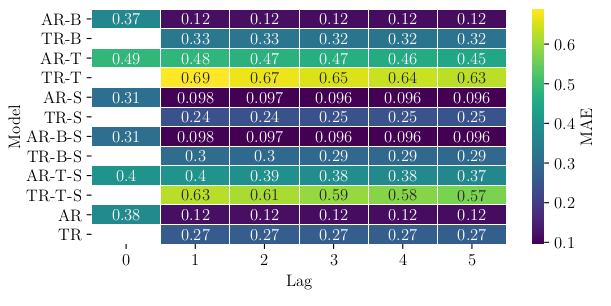
\includegraphics{python_figs/heat_ar_model_score.png} %\textbf{same colormap as MAE or obly for grids} 
    \caption{Heatmap showing the the performance of AR models averaged over all pixels.}
    \label{fig:results_ar_models}
\end{figure}
% se ark + flytt over bilde 
Figure \ref{fig:grid_mse_best_model} show the score of each pixel in the best model. Table \ref{tab:weights_best_model} provide the statisics of the weights in this model.
\begin{figure}
    \centering
    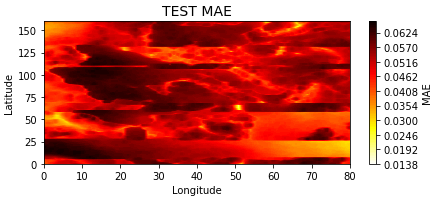
\includegraphics{python_figs/TEST_tcc.png}
    \caption{Grid showing the best models performance for all individual pixels. \textbf{Update this to be the best model}. Feilen her ligger i at latitude longitude informasjone er lagret som string i nc filene og sorteres derfor ikke når det leses inn pixelvis til et dataset. FIX dette kun for den beste modellen.}
    \label{fig:grid_mse_best_model}
\end{figure}

\begin{table}[hp]
    \centering
    \resizebox{\textwidth}{!}{%
    \begin{tabular}{cccccc}
    \cline{2-6}
     & \textbf{W1} & \textbf{W2} & \textbf{W3} & \textbf{W4} & \textbf{W5} \\ \hline
    %\textbf{Best model} & 0.3424 & 0.5 & 0.439839   & 0.83247 & 0.98347984 \\ \hline
    \textbf{Mean} & 0.3424 & 0.5 & 0.439839   & 0.83247 & 0.98347984 \\ \hline
    \textbf{Min} & 0.3424 & 0.5 & 0.439839   & 0.83247 & 0.98347984 \\ \hline
    \textbf{Max} & 0.3424 & 0.5 & 0.439839   & 0.83247 & 0.98347984 \\ \hline
    \textbf{STD} & 0.3424 & 0.5 & 0.439839   & 0.83247 & 0.98347984 \\ \hline
    \textbf{Median} & 0.3424 & 0.5 & 0.439839   & 0.83247 & 0.98347984 \\ \hline
    \end{tabular}%
    }
    \caption{Update the statistics of the best AR-model. \textbf{Ville det vært interresant?}}
    \label{tab:weights_best_model}
\end{table}

\subsection{Convolutional LSTM (ConvLSTM)}
The formulation of the air quality forecasting problem presented by \citeauthor{SunAirLSTM} is similar to the formulation of the cloud fractional cover forecasting problem presented in this study. 
%The machine learning experimental setup is adopted from the paper \citepaper{SunAirLSTM}.
% Endrer på arkitekturen - denne bruker -train - validation - test, en hvis prosentandel a

Architectural decisions %such as batch size, sequence length, number of filters and number of layers 
can cause the \acrshort{gpu} to run out of memory, resulting in non-trainable models.
%In these cases the compiled model is not trainable. 
To circumvent related issues, the \acrshort{convlstm}-models in this study was tuned manually. The list of hyperparameter to tune when working with \acrshort{convlstm}-model is long. In the initial experiments conducted in this study a subset of them is tuned and the rest is kept constant.

The following section describe the tuned hyperparameters. The dataset is partitioned into subsets called batches. The batch size is the number of ``examples'' \textbf{egentlig sequences} a weight update is based on. Epochs describes the number of times the model loops over the entire dataset. The sequence length is the number of timestamps a model aims to learn to predict. Number of hidden states it the number of filters it learns in each layer, see Section \ref{sec:convolutional neural network} for a 

for description of hidden states. 
The filter size determines the number of neighbours influencing an activation. Using kernel 1x1 results in the state-to-state transitions, similar to \acrshort{ar}-models without interactions between adjacent pixels. A more detailed description on this is provided in Sections \ref{sec:convolutional neural network} to \ref{sec:convolutional_lstm}. 

This section describe the hyperparameters kept constant. Between each \acrshort{convlstm}-layer there is a Batch Normalization layer (with its default settings). According to the \citepaper{ioffe2015batch} this should simplify the training process. Padding same is applied to all layers, to make sure the input and output dimensions are the same. This is described in more detail in Section \ref{sec:padding}. The model returns a sequence. The input sequences are not shuffled. The output filter and kernal size is one to concatenate all the previous hidden states to one without altering the output dimension. This is necessary for the predictions made.

The weights was initialized based on the scheme ``LeCun uniform'', see paper for more descriptions (\cite{Lecun98efficientbackprop}). Callbacks such as early stopping with patience of 10 epochs and terminate on NaN's have been applied to avoid prolonged training time. The optimizer ADAM (\cite{Kingma2015Adam:Optimization}) is used with the following settings, $\text{learning rate}=0.001$, $\text{beta1}=0.9$, $\text{beta2}=0.999$, $\text{epsilon}=1e-07$. The only difference from the default settings in Tensorflow is epsilon not being $1e-08$. The loss function is \acrfull{mse}, and the models are evaluate based on \acrfull{mae}.
Both functions are described in more detail in Section \ref{sec:metrics}. %The main difference between these functions is that \acrshort{mse} penalize points further away. This has its advantages in training the model, but makes it more difficult to interpret the results. The squared numbers in the range 0 to 1 shrink.

\subsubsection{Experimental setup (ConvLSTM)}
Models are given names based on an extension of the convention from \citepaper{precip_nowcasting}, ConvLSTM-hidden states-filter$\times$filter. 
% Trenge kanskje ikke nevne hva de hadde..?
By including batch size and sequence length the resulting naming convention becomes \newline $ConvLSTM-B_{x}-SL_{y}-hidden states-filter$\times$filter$. Table \ref{tab:convlstm_config} provide a set of example to hopefully clear any confusion.

\begin{table}[hp]
    \centering
    \resizebox{\textwidth}{!}{%
    \begin{tabular}{ccccc}
     \textbf{ConvLSTM Model} & \textbf{Sequence Length} & \textbf{Batch Size} & \textbf{Hidden States} & \textbf{Kernels} \\ \hline
    \textbf{$B_{5}-SL_{24}$ \newline $-256-3\times3-256-3\times3$} & 24 & 5 & [256, 256]   & [3, 3] \\ \hline
    \textbf{$B_{15}-SL_{24}-256-5\times5-256-5\times5$} & 24 & 15 & [256, 256]  & [5, 5] \\ \hline
    \textbf{$B_{10}-SL_{24}-128-1\times1-128-1\times1$} & 24 & 10 &  [128, 128] & [1, 1] \\ \hline
    \textbf{$B_{5}-SL_{6}-64-3\times3-64-3\times3$} & 6 & 5 & [64, 64] & [3, 3] \\ \hline
    \textbf{$B_{5}-SL_{6}-256-3\times3-256-3\times3$} & 6 & 5 & [64, 32] & [3, 3] \\ \hline
    \textbf{$B_{5}-SL_{6}-8-3\times3-8-3\times3-8-3\times3$} & 6 & 5 & [8, 8, 8] & [3, 3, 3] \\ \hline
    \end{tabular}%
    }
    \caption{Examples to simplify the explanation of configurations and models.}
    \label{tab:convlstm_config}
\end{table}

Figure \ref{fig:convlstm_loss} show the loss curves in the training process for all the compiled models in this study. The training loss is higher than the validation loss since there is a higher number of samples in the training set than the validation set and it is not scaled.

\begin{figure}
    \centering
    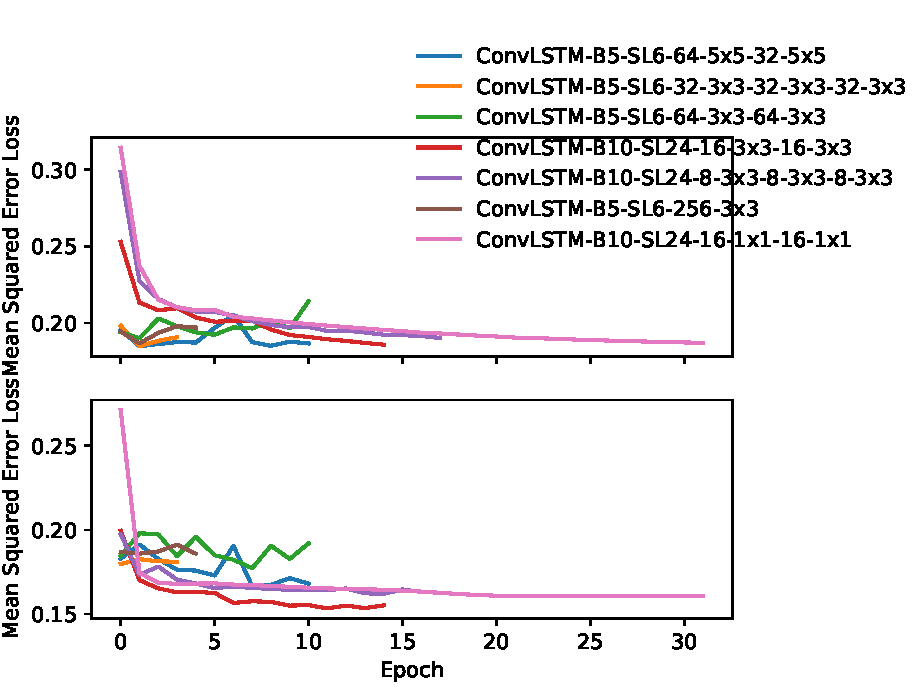
\includegraphics{python_figs/test_epoch_loss.pdf}
    \caption{Loss vs epochs for the trained models in this thesis. Subplot train and valid loss. The resulting legend is then only the model names.}
    \label{fig:convlstm_loss}
\end{figure}
%List of non-trainable models attempted:
As a reference to future studies below is a listing of non-trainable architectures.
\begin{enumerate}
    \item $ConvLSTM-B_{10}-SL_{24}-128-3\times3$
    \item $ConvLSTM-B_{10}-SL_{24}-128-3\times3-32-3\times3$
    \item $ConvLSTM-B_{10}-SL_{24}-64-3\times3-64-3\times3$
    \item $ConvLSTM-B_{5}-SL_{24}-256-3\times3-256-3\times3$
    \item $ConvLSTM-B_{5}-SL_{6}-256-3\times3-256-3\times3$
\end{enumerate}

%%%%%%%%%%%%%%%%%%%%%%%%% The copied dictionary is the result from tf.evaluate. 
\begin{table}[]
    \centering
    \resizebox{\textwidth}{!}{
    \begin{tabular}{c|lccc}
    \textbf{ConvLSTM Model} & \textbf{Train Loss} & \textbf{Val Loss} & \textbf{Test Loss} & \textbf{Num. Params.} \\ \hline 
    \rowcolor{cyan!15}
    $B_{10}-SL_{24}-16-3\times3-16-3\times3$ &  &  &  &  30 296\\ \hline
    % {"loss": 0.15752051770687103, "mean_squared_error": 0.15752056241035461, "r2_keras": 0.15506696701049805, "mean_absolute_error": 0.34570422768592834}
    
    $B_{10}-SL_{24}-16-1\times1-16-1\times1$ &  &  &  &  \\ \hline
    
    $B_{10}-SL_{24}-32-1\times1-32-1\times1$ & 0.16490 &  & 0.350855 &  \\ \hline
    % {"loss": 0.1649022251367569, "mean_squared_error": 0.1649022400379181, "r2_keras": 0.1159096509218216, "mean_absolute_error": 0.35085538029670715}
    
    $B_{10}-SL_{24}-32-3\times3-32-3\times3$ &  &  &  &  \\ \hline
    %{"loss": 0.15340088307857513, "mean_squared_error": 0.15340085327625275, "r2_keras": 0.17754235863685608, "mean_absolute_error": 0.33814743161201477}
    
    $B_{10}-SL_{24}-32-5\times5-32-5\times5$ &  &  &  &  \\ \hline
    % {"loss": 0.15889282524585724, "mean_squared_error": 0.15889279544353485, "r2_keras": 0.147248774766922, "mean_absolute_error": 0.34079509973526}
    
    $B_{10}-SL_{24}-8-3\times3-8-3\times3-8-3\times3$ &  &  &  &  \\ \hline
    % {"loss": 0.16335555911064148, "mean_squared_error": 0.16335561871528625, "r2_keras": 0.12448494136333466, "mean_absolute_error": 0.3477591276168823}
    
    $B_{10}-SL_{24}-32-5\times5-32-5\times5$ &  &  &  &  \\ \hline
    %{"loss": 0.1632702797651291, "mean_squared_error": 0.16327014565467834, "r2_keras": 0.09565786272287369, "mean_absolute_error": 0.3411720395088196}
    
    $B_{10}-SL_{24}-256-3\times3$ &  &  &  &  \\ \hline
    $B_{5}-SL_{6}-64-3\times3-64-3\times3$ &  &  &  &  \\ \hline
    $B_{5}-SL_{6}-64-5\times5-64-5\times5$ &  &  &  &  \\ \hline
    
    \end{tabular}
    }
    \caption{Results, metrics and number of parameters for the trained models. The best model \acrshort{convlstm}-model is highlighted in light blue.}
    \label{tab:convlstmLoss}
\end{table}

\textbf{Comment on the difference using a filter 1 by 1, and excluding the spatial relation in the model.}

\begin{figure}
    \centering
    %
\tikzset{every picture/.append style={scale=1.0}}
\begin{tikzpicture}[x={(1,0)},y={(0,1)}, z={({cos(60)},{sin(60)})},
font=\sffamily\small, scale=1.0]

\tikzset{pics/fake box/.style args={% #1=color, #2=x dimension, #3=y dimension, #4=z dimension
#1 with dimensions #2 and #3 and #4}{
code={
\draw[teal,ultra thin,fill=#1,opacity=0.25]  (0,0,0) coordinate(-front-bottom-left) to
++ (0,#3,0) coordinate(-front-top-right) --++
(#2,0,0) coordinate(-front-top-right) --++ (0,-#3,0) 
coordinate(-front-bottom-right) -- cycle;
\draw[teal,ultra thin,fill=#1, opacity=0.25] (0,#3,0)  --++ 
 (0,0,#4) coordinate(-back-top-left) --++ (#2,0,0) 
 coordinate(-back-top-right) --++ (0,0,-#4)  -- cycle;
\draw[teal,ultra thin,fill=#1!80!black, opacity=0.25] (#2,0,0) --++ (0,0,#4) coordinate(-back-bottom-right)
--++ (0,#3,0) --++ (0,0,-#4) -- cycle;
\path[teal,decorate,decoration={text effects along path,text={}}] (#2/2,{3.4+(#3-2)/2},0) -- (#2/2,0,0);
}
}}

%%%%%%%%%% Green box in the back symbolizing batches 
\foreach \X / \Y in {2.3/-1.5} {
\draw pic (box1-\Y) at (\Y,-\X/,0) {fake box=green with dimensions 14.6 and {2*\X} and 1*\X};
}


%%%%%%%%%%%%%%%%%%%%%%%%%%%%%% BLUE BOX
\foreach \X / \Y in {1.5/-1.0, 1.5/6} {
\draw pic (box1-\Y) at (\Y,-\X/,0) {fake box=white!25!cyan with dimensions 6.9 and {2*\X} and 1*\X};
}


%%%%%%%%%%%%%%%%%%%%%%%%%%%%%%% Weather data volume 1.
\foreach \X/\Col in {0.0/red, 0.2/green, 0.4/cyan, 0.6/yellow} %{6.5/red,6.7/green,6.9/blue}
{\draw[canvas is yz plane at x = \X, transform shape, draw = black, fill = \Col!50!white, opacity = 0.5] (0,0.5) rectangle (2,-1.5);}

%\draw[gray!60,thick] (-0.1,-0.1,-1.6) coordinate (1-1) -- (-0.1,-0.1,0.6) coordinate (1-2) -- (-0.1, 2.,0.6) coordinate (1-3) -- (-0.1, 2.1,-1.6) coordinate (1-4) -- cycle;

%\draw[gray!60,thick] (0.8,-0.1,-1.6) coordinate (2-1) -- (0.8,-0.1,0.6) coordinate (2-2) -- (0.8, 2.,0.6) coordinate (2-3) -- (0.8,2.1,-1.6) coordinate (2-4) -- cycle;

%\foreach \X in {4,1,3}{\draw[gray!60,thick] (1-\X) -- (2-\X);}

\tikzset{pics/fake box/.style args={% #1=color, #2=x dimension, #3=y dimension, #4=z dimension
#1 with dimensions #2 and #3 and #4}{
code={
\draw[teal,ultra thin]  (0,0,0) coordinate(-front-bottom-left) to
++ (0,#3,0) coordinate(-front-top-right) --++
(#2,0,0) coordinate(-front-top-right) --++ (0,-#3,0) 
coordinate(-front-bottom-right) -- cycle;
\draw[teal,ultra thin] (0,#3,0)  --++ 
 (0,0,#4) coordinate(-back-top-left) --++ (#2,0,0) 
 coordinate(-back-top-right) --++ (0,0,-#4)  -- cycle;
\draw[teal,ultra thin,fill=#1!80!black] (#2,0,0) --++ (0,0,#4) coordinate(-back-bottom-right)
--++ (0,#3,0) --++ (0,0,-#4) -- cycle;
\path[teal,decorate,decoration={text effects along path,text={}}] (#2/2,{3.4+(#3-2)/2},0) -- (#2/2,0,0);
}
}}

%%%%%%%%%%%%%%%%%%%%%%%%%%%%%%%%%%%%%%%%%%%%

%%%%%%%%%%%%%%%%%%%%%%%%%%%%%% BLUE BOX

\foreach \X/\Col in {2.0/red,2.2/green,2.4/cyan, 2.6/yellow} %{6.5/red,6.7/green,6.9/blue}
{\draw[canvas is yz plane at x = \X, transform shape, draw = black, fill = \Col!50!white, opacity = 0.5] (0,0.5) rectangle (2,-1.5);}

\foreach \X/\Col in {5.0/red,5.2/green,5.4/cyan, 5.6/yellow} %{6.5/red,6.7/green,6.9/blue}
{\draw[canvas is yz plane at x = \X, transform shape, draw = black, fill = \Col!50!white, opacity = 0.5] (0,0.5) rectangle (2,-1.5);}

%%%%%%%%%%%%%%% Second bow
\foreach \X/\Col in {7.0/red,7.2/green,7.4/cyan, 7.6/yellow} %{6.5/red,6.7/green,6.9/blue}
{\draw[canvas is yz plane at x = \X, transform shape, draw = black, fill = \Col!50!white, opacity = 0.5] (0,0.5) rectangle (2,-1.5);}

\foreach \X/\Col in {9.0/red,9.2/green,9.4/cyan, 9.6/yellow} %{6.5/red,6.7/green,6.9/blue}
{\draw[canvas is yz plane at x = \X, transform shape, draw = black, fill = \Col!50!white, opacity = 0.5] (0,0.5) rectangle (2,-1.5);}

\foreach \X/\Col in {12.0/red,12.2/green,12.4/cyan, 12.6/yellow} %{6.5/red,6.7/green,6.9/blue}
{\draw[canvas is yz plane at x = \X, transform shape, draw = black, fill = \Col!50!white, opacity = 0.5] (0,0.5) rectangle (2,-1.5);}

%%%%%%%%%%%%%%%%%%% ADDING TEXT
\node[color = gray, thick] at (6, 3.3) {\Large Batch \#0};
\node[color = blue!60, thick] at (1.0, -2.0) {\large SEQUENCE \#0};
\node[color = blue!60, thick] at (8.0, -2.0) {\large SEQUENCE \#1};
\node[color = gray, thick, rotate=60] at (0.3, 0.1) {$00:00$};
\node[color = gray, thick, rotate=60] at (2.3, 0.05) {$01:00$};
\node[color = gray, thick, rotate=60] at (5.3, 0.0) {$23:00$};

\node[color = gray, thick, rotate=60] at (7.3, 0.1) {$00:00$};
\node[color = gray, thick, rotate=60] at (9.3, 0.05) {$01:00$};
\node[color = gray, thick, rotate=60] at (12.3, 0.0) {$23:00$};


%%%%%%%%%%%%%% Dotted lines
\path[draw, thick, dotted] (3.0, 0.5) edge (4., 0.5);
\path[draw, thick, dotted] (10.0, 0.5) edge (11., 0.5);

\end{tikzpicture}
%\end{document}

    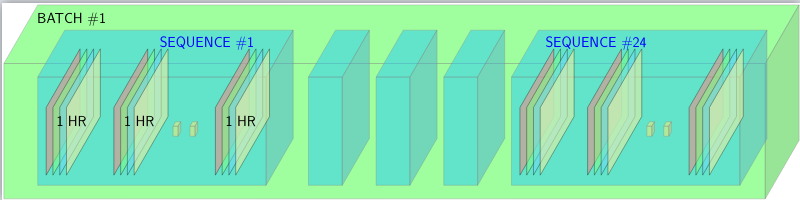
\includegraphics[scale=0.6]{ChapterX_Results_and_Conclusion/computational_experiments/temp_input_volume.png}
    \caption{Illustration of the content of the first batch. A batch is a 5-dimensional data volume. For each hour the weather data volume is $81\times 161\times 4$, a sequence consist of 24 of these volumes and a batch contain 10 sequences. \ref{fig:best_ml_architecture} \textbf{Comment to Trude, I have drawn this in tikz, and will include the code, due to some scaling issues I've used the screenshot to comments on.}}
    \label{fig:input_volume_conv_lstm}
\end{figure}

The best performing \acrshort{convlstm}-model is the $ConvLSTM-B_{10}-SL_{24}-16-3\times3-16-3 times3$. It architecture is shown in Figure \ref{fig:best_ml_architecture}, the input volume is currently very simplified. The real input volume is provided in Figure \ref{fig:input_volume_conv_lstm}. 

\begin{figure}
    \centering
    \begin{tikzpicture}[x={(1,0)},y={(0,1)},z={({cos(60)},{sin(60)})},
font=\sffamily\small,scale=1.9] % 1.7 passer bra på siden.

\tikzset{circle dotted/.style={dash pattern=on .05mm off 2mm,
                                         line cap=round}}

%
% comment these out if you want to see where the axes point to
% \draw[-latex] (0,0,0) -- (3,0,0) node[below]{$x$};
% \draw[-latex] (0,0,0) -- (0,3,0) node[left]{$y$};
% \draw[-latex] (0,0,0) -- (0,0,3) node[below]{$z$};
% a plane
\tikzset{pics/fake box/.style args={% #1=color, #2=x dimension, #3=y dimension, #4=z dimension
#1 with dimensions #2 and #3 and #4}{
code={
\draw[teal,ultra thin,fill=#1]  (0,0,0) coordinate(-front-bottom-left) to
++ (0,#3,0) coordinate(-front-top-right) --++
(#2,0,0) coordinate(-front-top-right) --++ (0,-#3,0) 
coordinate(-front-bottom-right) -- cycle;
\draw[teal,ultra thin,fill=#1] (0,#3,0)  --++ 
 (0,0,#4) coordinate(-back-top-left) --++ (#2,0,0) 
 coordinate(-back-top-right) --++ (0,0,-#4)  -- cycle;
\draw[teal,ultra thin,fill=#1!80!black] (#2,0,0) --++ (0,0,#4) coordinate(-back-bottom-right)
--++ (0,#3,0) --++ (0,0,-#4) -- cycle;
\path[teal,decorate,decoration={text effects along path,text={BATCH NORM}}] (#2/2,{3.4+(#3-2)/2},0) -- (#2/2,0,0);
}
}}
%3.0/1.5, 3.0/3.3, 3.0/5.0
\foreach \X / \Y in {3.0/1.3, 3.0/3., 3.0/4.6} 
%2.2,2.2,2.0
{
\draw pic (box1-\Y) at (\Y,-\X/2,0) {fake box=white!70!teal with dimensions 0.5 and {2*\X} and 1*\X};
}

%%%%%%%%%%%%%%%%%%%%%%%%%%%%%%%%%%%% 
\tikzset{pics/fake box/.style args={% #1=color, #2=x dimension, #3=y dimension, #4=z dimension
#1 with dimensions #2 and #3 and #4}{
code={
\draw[gray,ultra thin,fill=#1]  (0,0,0) coordinate(-front-bottom-left) to
++ (0,#3,0) coordinate(-front-top-right) --++
(#2,0,0) coordinate(-front-top-right) --++ (0,-#3,0) 
coordinate(-front-bottom-right) -- cycle;
\draw[gray,ultra thin,fill=#1] (0,#3,0)  --++ 
 (0,0,#4) coordinate(-back-top-left) --++ (#2,0,0) 
 coordinate(-back-top-right) --++ (0,0,-#4)  -- cycle;
\draw[gray,ultra thin,fill=#1!80!black] (#2,0,0) --++ (0,0,#4) coordinate(-back-bottom-right)
--++ (0,#3,0) --++ (0,0,-#4) -- cycle;
\path[gray,decorate,decoration={text effects along path,text={CONV LSTM}}] (#2/2,{3.4+(#3-2)/2},0) -- (#2/2,0,0);
}
}}

%%%%%%%%%%%%%%%%%%%%%%%%%%%%%%
\foreach \X / \Y in {3.0/1.6, 3.0/3.3, 3.0/4.9}
%2.2,2.2,2.0
{
\draw pic (box1-\Y) at (\Y,-\X/2,0) {fake box=white!70!gray with dimensions 0.5 and {2*\X} and 1*\X};
}

%\foreach \X/\Col in {0.0/red,0.2/green,0.4/cyan, 0.6/yellow, 6.8/blue} %{6.5/red,6.7/green,6.9/blue}
%{\draw[canvas is yz plane at x = \X, transform shape, draw = black, fill = \Col!50!white, opacity = 0.5] (0,0.5) rectangle (2,-1.5);}

%\draw[gray!60,thick] (-0.1,-0.1,-1.6) coordinate (1-1) -- (-0.1,-0.1,0.6) coordinate (1-2) -- (-0.1, 2.,0.6) coordinate (1-3) -- (-0.1, 2.1,-1.6) coordinate (1-4) -- cycle;
%\draw[gray!60,thick] (0.8,-0.1,-1.6) coordinate (2-1) -- (0.8,-0.1,0.6) coordinate (2-2) -- (0.8, 2.,0.6) coordinate (2-3) -- (0.8,2.1,-1.6) coordinate (2-4) -- cycle;

%%%%%%%%%%%%%%%%%%%%%%%%%%%%%%%%%%%% 
\tikzset{pics/fake box/.style args={% #1=color, #2=x dimension, #3=y dimension, #4=z dimension
#1 with dimensions #2 and #3 and #4}{
code={
\draw[gray,ultra thin,fill=#1]  (0,0,0) coordinate(-front-bottom-left) to
++ (0,#3,0) coordinate(-front-top-right) --++
(#2,0,0) coordinate(-front-top-right) --++ (0,-#3,0) 
coordinate(-front-bottom-right) -- cycle;
\draw[gray,ultra thin,fill=#1] (0,#3,0)  --++ 
 (0,0,#4) coordinate(-back-top-left) --++ (#2,0,0) 
 coordinate(-back-top-right) --++ (0,0,-#4)  -- cycle;
\draw[gray,ultra thin,fill=#1!80!black] (#2,0,0) --++ (0,0,#4) coordinate(-back-bottom-right)
--++ (0,#3,0) --++ (0,0,-#4) -- cycle;
\path[gray,decorate,decoration={text effects along path,text={INPUT}}] (#2/2,{2.4+(#3-2)/2},0) -- (#2/2,0,0);
}
}}

%%%%%%%%%%%%%%%%%%%%%%%%%%%%%%
\foreach \X / \Y in {3.0/-1.0}
%2.2,2.2,2.0
{
\draw pic (box1-\Y) at (\Y,-\X/2,0) {fake box=white!70!green with dimensions 2.5 and {2*\X} and 1*\X};
}

\tikzset{pics/fake box/.style args={% #1=color, #2=x dimension, #3=y dimension, #4=z dimension
#1 with dimensions #2 and #3 and #4}{
code={
\draw[gray,ultra thin,fill=#1]  (0,0,0) coordinate(-front-bottom-left) to
++ (0,#3,0) coordinate(-front-top-right) --++
(#2,0,0) coordinate(-front-top-right) --++ (0,-#3,0) 
coordinate(-front-bottom-right) -- cycle;
\draw[gray,ultra thin,fill=#1] (0,#3,0)  --++ 
 (0,0,#4) coordinate(-back-top-left) --++ (#2,0,0) 
 coordinate(-back-top-right) --++ (0,0,-#4)  -- cycle;
\draw[gray,ultra thin,fill=#1!80!black] (#2,0,0) --++ (0,0,#4) coordinate(-back-bottom-right)
--++ (0,#3,0) --++ (0,0,-#4) -- cycle;
\path[gray,decorate,decoration={text effects along path,text={OUTPUT}}] (#2/2,{2.6+(#3-2)/2},0) -- (#2/2,0,0);
}
}}

\foreach \X / \Y in {3.0/6.1}
%2.2,2.2,2.0
{
\draw pic (box1-\Y) at (\Y,-\X/2,0) {fake box=white!70!blue with dimensions 1.0 and {2*\X} and 1*\X};
}

%\foreach \X in {4,1,3}
%{\draw[gray!60,thick] (1-\X) -- (2-\X);}

\node[draw,single arrow, orange,fill=orange!30] at (0.8, 0.5,0) {BATCH};
\node[draw,single arrow, orange,fill=orange!30] at (2.4, 0.5,0) {$3\times 3$};
\node[draw,single arrow, orange,fill=orange!30] at (4., 0.5,0) {$3\times 3$};
\node[draw,single arrow, orange,fill=orange!30] at (5.6, 0.5,0) {$1\times 1$};

%\begin{scope}[on background layer]
%\node[orange,thick,rounded corners,fill=orange!30,fit=(A1) (A3)]{};
%\node[gray,thick,rounded corners,fill=gray!10,fit=(B1) (B3)]{};
%\end{scope}

%\foreach \X in {1,2,3}
%{\draw[-latex] (A\X) -- (B2);}

\draw[thick](0.2, 3.3)node[scale=1.]{\small $10\times 24\times 81\times 161 \times 4 $};
\draw[thick](1.5, -2)node[scale=1.]{\small $10\times 24\times81\times 161 \times 32 $};
\draw[thick](3.8, 3.3)node[scale=1.]{\small $10\times 24\times 81\times 161 \times 32 $};
\draw[thick](5.0, -2)node[scale=1.]{\small $10\times 24\times 81\times 161 \times 1 $};
\draw[thick](6.6, 3.3)node[scale=1.]{\small $10\times 24\times 81\times 161 \times 1 $};
\end{tikzpicture}
    \caption{The architecture of the cloud cover forecasting model developed in this study. The content of the input volume is displayed in Figure \ref{fig:input_volume_conv_lstm}, 16 hidden states in each \acrshort{convlstm} layer and $3\times 3$ kernel. The output layer has one hidden state and the kernel dimension of $1\times 1$ kernel.
    The input shape is 10x24x81x161x4 and output 24x81x161x1.  }
    \label{fig:best_ml_architecture}
\end{figure}

Of the predicted sequence 2014-2018 $0.5\%$ is below zero (never below -1) but non is above 1. %17140/3129840 = 0.005476318278250646

\subsection{Results on Predicting sequence}
The foundation of the choice of the best model is different for \acrshort{ar} and \acrshort{convlstm}-models. As mentioned in Chapter \ref{ch:num_methods}, the \acrshort{ar}-model is optimized to fit the next timestep, while the \acrshort{convlstm} is optimised to fit a sequence or a prescribed length. In this section the best \acrshort{ar}-model and \acrshort{convlstm}-model are assessed on how well they predict the sequence length of the best \acrshort{convlstm}-model. By feeding the prediction into the \acrshort{ar}-model, one can modify its ability to predict sequences. The two best models are X and Y, with performance measured by the MAE metric of A and B respectively. 

%\subsubsection{Visual Comparison predicting a sequence of length}
Visualizing the experiments for sequences.
%%%% TARGET PREDICITON ERA5
\begin{figure}[ht]
    \centering
    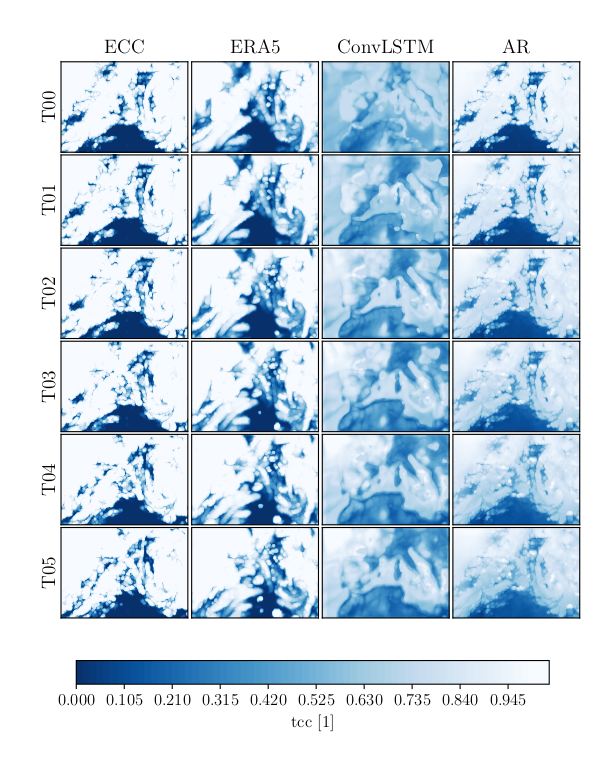
\includegraphics[sale=0.1]{python_figs/comparting_seq_part_1_of4.png}
    \caption{First of 4 part since the sequence is 24 hours long, the full series of plots for this sequence can be found in Appendix \ref{app:pred_sequence} }
    \label{fig:target_predict_era5_horizontal}
\end{figure}

Some text where you comment the results from this comparison. Is it evident that the \acrshort{convlstm} is better at predicting spatial patterns as expected or does it all resemble random noise. Is the predicted values in sample or out of sample.


\subsection{Summary} \label{sec:summary_num}
Add text ... 

\clearpage
\section{Practical implications - OUTDATED} \label{sec:practical_implications}
It is necessary to have a understanding of the needs of the end product before conducting large machine learning projects. Answering questions like: What will it be used for and how can it be implemented in useful way?

A major downside of the data driven learning approach is the rigid resolution. A trained model can only be used on similar problems, with the same spatiotemporal resolution. For applications like climate models, output comes in a wide range of different resolutions. Before implementing the finished product in a new model of a different resolution, it would need to be retrained on the resolution of the climate model under development. This process involves both remapping of the dataset and retraining the model at the correct resolution. This is a time consuming process involving finding a new set of hyperparameters suitable for the new resolution. % It essentially means starting over.

Once trained on global climate datasets, machine learning models provide fast results even for complex parameterization which is what makes them suitable for the application of climate modelling. Most machine learning packages are developed using Python. \acrfull{esm} are implemented in python. Methods for including the trained parameterizations need to be developed.
 
\subsection{Any implications based on the results presented in this chapter.}